\subsection{Phân hệ Thông báo}
\label{subsec:req_notification}
\label{subsec:module_notification}

\subsubsection{Mục tiêu}
Phân hệ Thông báo cung cấp một điểm tiếp nhận thông tin và sự kiện nghiệp vụ tập trung trên ứng dụng di động cho toàn bộ các dịch vụ HRM và iOffice.

Mục tiêu của phân hệ không chỉ dừng lại ở việc hiển thị các biểu ngữ (banner) thông báo đẩy tức thời, mà còn hỗ trợ người dùng nhận diện ngữ cảnh nghiệp vụ và kích hoạt cơ chế điều hướng sâu (Deep Linking) trực tiếp đến đúng màn hình đối tượng cần xử lý trên ứng dụng.

\subsubsection{Yêu cầu chức năng}

\begin{itemize}[leftmargin=1.5cm]
    \item \textbf{FR-NOT-01 -- Đăng ký thiết bị nhận thông báo:} Sau khi người dùng đăng nhập thành công và thiết bị được cấp FCM Device Token từ dịch vụ Firebase, ứng dụng Mobile phải tự động gửi token này lên backend để liên kết với tài khoản người dùng hiện tại.
    
    \item \textbf{FR-NOT-02 -- Cập nhật token:} Khi dịch vụ FCM làm mới hoặc cấp lại token cho thiết bị, ứng dụng phải tự động phát hiện và gửi token mới lên backend để cập nhật thông tin tiếp nhận.
    
    \item \textbf{FR-NOT-03 -- Nhận thông báo:} Ứng dụng phải hỗ trợ tiếp nhận thông báo đẩy trong mọi trạng thái hoạt động của thiết bị (Foreground, Background, Terminated) phù hợp với cơ chế của hệ điều hành Android và iOS.
    
    \item \textbf{FR-NOT-04 -- Xem trung tâm thông báo:} Người dùng có thể mở Trung tâm thông báo trên ứng dụng để xem danh sách toàn bộ các thông báo đã nhận, phân biệt rõ ràng giữa thông báo đã đọc và chưa đọc.
    
    \item \textbf{FR-NOT-05 -- Cập nhật trạng thái đọc:} Khi người dùng mở xem thông báo hoặc thực hiện thao tác đánh dấu đã đọc, hệ thống phải cập nhật trạng thái tương ứng trên giao diện và gửi request đồng bộ về backend.
    
    \item \textbf{FR-NOT-06 -- Điều hướng theo ngữ cảnh (Deep Linking):} Khi người dùng chạm vào một thông báo có dữ liệu định tuyến hợp lệ, ứng dụng phải trích xuất các trường thông tin chuẩn hóa để xác định chính xác màn hình cần mở:
\end{itemize}

\begin{table}[H]
\centering
\renewcommand{\arraystretch}{1.25}
\begin{tabularx}{\textwidth}{|p{3.5cm}|X|}
\hline
\textbf{Trường Metadata} & \textbf{Ý nghĩa nghiệp vụ phục vụ định tuyến} \\
\hline
\texttt{source} & Miền dịch vụ phát sinh thông báo (ví dụ \texttt{'hrm'} hoặc \texttt{'ioffice'}). \\
\hline
\texttt{entityType} & Loại đối tượng nghiệp vụ (\texttt{'leave'}, \texttt{'business-trip'}, \texttt{'incoming-doc'}, \texttt{'outgoing-doc'}, \texttt{'task'}). \\
\hline
\texttt{entityId} & Khóa chính định danh duy nhất của bản ghi đối tượng cần mở (ID đơn nghỉ phép, ID nhiệm vụ...). \\
\hline
\texttt{isApproval} & Cờ đánh dấu ngữ cảnh: \texttt{true} nếu cần mở giao diện phê duyệt của cấp quản lý, \texttt{false} nếu mở giao diện xem chi tiết thông thường. \\
\hline
\end{tabularx}
\caption{\textit{Chuẩn hóa các trường Metadata định tuyến thông báo}}
\label{tab:notification_metadata}
\end{table}

\begin{itemize}[leftmargin=1.5cm]
    \item \textbf{FR-NOT-07 -- Xử lý thông báo không còn hợp lệ:} Trường hợp đối tượng được thông báo tham chiếu đã bị xóa, người dùng không còn quyền truy cập hoặc route điều hướng không xác định được, ứng dụng tuyệt đối không được điều hướng tới một màn hình sai hoặc làm dừng đột ngột ứng dụng; hệ thống phải hiển thị thông báo giải thích nhẹ nhàng và giữ người dùng ở trạng thái an toàn.
    
    \item \textbf{FR-NOT-08 -- Đăng xuất thiết bị:} Khi người dùng đăng xuất, ứng dụng phải gửi request yêu cầu backend hủy liên kết giữa FCM token của thiết bị và tài khoản người dùng, nhằm ngăn chặn triệt để nguy cơ gửi thông báo nghiệp vụ của người dùng cũ đến thiết bị.
\end{itemize}

\subsubsection{Đặc tả Ca sử dụng (Use Cases)}

\usecasespec{
  id={UC-NOT-01},
  name={Xem và mở thông báo},
  actor={Người dùng ứng dụng MyHCMUT Mobile.},
  pre={Người dùng đã đăng nhập vào ứng dụng.},
  trigger={Người dùng mở Trung tâm thông báo hoặc chạm vào thông báo đẩy xuất hiện trên màn hình khóa / thanh trạng thái.},
  mainflow={
    1. Hệ thống lấy danh sách thông báo và hiển thị trạng thái đã đọc/chưa đọc. \newline
    2. Người dùng chọn một mục thông báo cụ thể. \newline
    3. Ứng dụng đánh dấu thông báo là đã đọc và phân tích 4 trường metadata (\texttt{source}, \texttt{entityType}, \texttt{entityId}, \texttt{isApproval}). \newline
    4. Hệ thống xác định đường dẫn điều hướng (Route) tương ứng và kích hoạt chuyển màn hình trực tiếp đến đúng đối tượng nghiệp vụ.
  },
  altflow={
    Metadata không hợp lệ hoặc bản ghi đối tượng đã bị xóa $\rightarrow$ Hệ thống hiển thị thông báo đối tượng không khả dụng và không thực hiện điều hướng sai.
  },
  post={Người dùng được đưa tới đúng ngữ cảnh cần thao tác; trạng thái thông báo được cập nhật là Đã đọc.},
  label={tab:uc_not_01}
}

\usecasespec{
  id={UC-NOT-02},
  name={Quản lý token thiết bị},
  actor={Ứng dụng Mobile (thực thi tự động dưới nền).},
  trigger={Người dùng đăng nhập thành công, FCM token được làm mới, hoặc người dùng đăng xuất.},
  mainflow={
    1. Ứng dụng nhận FCM Device Token từ dịch vụ Google Firebase. \newline
    2. Gửi request kèm token và định danh người dùng lên backend dịch vụ thông báo. \newline
    3. Backend kiểm tra và cập nhật bản ghi ánh xạ giữa \texttt{user\_id} và \texttt{device\_token} trong bảng dữ liệu thiết bị. \newline
    4. Khi người dùng đăng xuất, ứng dụng gửi lệnh thu hồi để backend hủy kích hoạt token tương ứng.
  },
  post={Cơ sở dữ liệu backend duy trì danh sách các token thiết bị đang hoạt động hợp lệ cho người dùng.},
  label={tab:uc_not_02}
}

\subsubsection{Quy tắc nghiệp vụ (Business Rules)}

\begin{itemize}[leftmargin=1.5cm]
    \item \textbf{BR-NOT-01:} Người dùng chỉ được phép truy xuất và thao tác trên danh sách các thông báo thuộc quyền sở hữu của chính tài khoản mình.
    \item \textbf{BR-NOT-02:} Toàn bộ dữ liệu metadata điều hướng gửi kèm thông báo phải được kiểm tra và chuẩn hóa trước khi tạo lệnh điều hướng; ứng dụng không được tin cậy hoàn toàn dữ liệu push như một lệnh điều hướng tự do.
    \item \textbf{BR-NOT-03:} Các tham số \texttt{source}, \texttt{entityType}, \texttt{entityId} và ngữ cảnh \texttt{isApproval} bắt buộc phải được ánh xạ sang các route nội bộ đã được định nghĩa tĩnh trong bộ định tuyến của ứng dụng.
    \item \textbf{BR-NOT-04:} Quyền truy cập vào đối tượng nghiệp vụ sau khi điều hướng sâu (Deep Link) vẫn phải được backend kiểm tra độc lập; việc nhận được thông báo không đồng nghĩa với việc tự động được cấp quyền thao tác.
    \item \textbf{BR-NOT-05:} FCM Device Token có thể thay đổi trong suốt vòng đời của ứng dụng; Mobile phải cài đặt cơ chế lắng nghe sự kiện làm mới token để kịp thời cập nhật lên máy chủ.
    \item \textbf{BR-NOT-06:} Khi dịch vụ Firebase FCM phản hồi thông báo về một token không còn hợp lệ (Unregistered / Invalid Token), backend phải tự động xóa hoặc gắn cờ vô hiệu hóa token đó trong cơ sở dữ liệu.
    \item \textbf{BR-NOT-07:} Tính năng hiển thị số đếm huy hiệu (Badge Counter) phụ thuộc hoàn toàn vào hệ điều hành và giao diện trình khởi chạy (Launcher) của từng dòng máy; hệ thống không cam kết mọi thiết bị đều hiển thị số badge đồng nhất.
    \item \textbf{BR-NOT-08:} Hệ thống không giả định rằng mọi sự kiện thông báo đẩy đều được phân phối tới thiết bị chính xác một lần (không bảo đảm Exactly-Once). Phân hệ thông báo chỉ đóng vai trò kênh hỗ trợ thông tin nhanh; trạng thái nghiệp vụ chuẩn mực cuối cùng luôn phải được truy vấn từ backend.
\end{itemize}

\subsubsection{Biểu đồ Tuần tự (Sequence Diagrams)}

\begin{figure}[H]
    \centering
    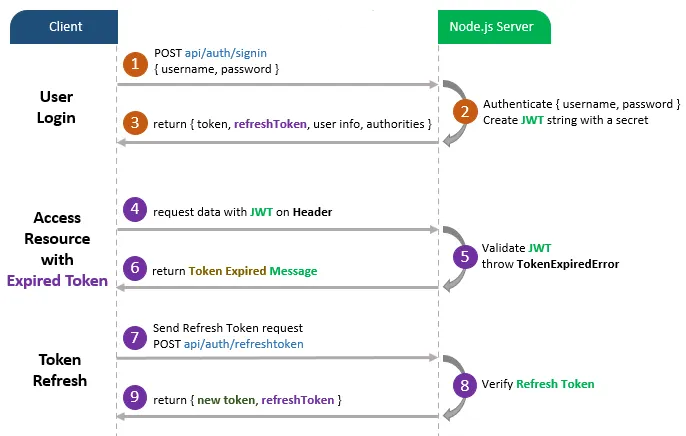
\includegraphics[width=0.85\linewidth]{img/uml/seq_kafka_fcm_push.png}
    \caption{\textit{Biểu đồ Tuần tự Pipeline Thông báo Đẩy Bất đồng bộ (Kafka sang FCM sang Mobile)}}
    \label{fig:seq_noti_kafka_fcm}
\end{figure}

Biểu đồ hình \ref{fig:seq_noti_kafka_fcm} thể hiện toàn bộ quy trình phát tán thông báo bất đồng bộ. Điểm mấu chốt trong thiết kế là việc tách biệt ranh giới giao dịch cơ sở dữ liệu với việc phát thông điệp vào Kafka: hàm phát tán chỉ được gọi sau khi lệnh \texttt{transaction.commit()} đã hoàn tất thành công. Nhờ đó, hệ thống ngăn chặn hoàn toàn hiện tượng người dùng nhận thông báo về một đơn từ hoặc quyết định đã bị hủy bỏ do lỗi giao dịch ở tầng cơ sở dữ liệu. Toàn bộ logic giải mã metadata và điều hướng sâu đã được kiểm thử tự động với 47 ca kiểm thử chuyên biệt cho module thông báo.
